This chapter is mainly dedicated to users currently running Ubuntu 10.04 LTS or 10.10 and are looking forward to upgrade to Ubuntu 12.04 LTS. Before you begin to ponder the need for this chapter, it is mainly to briefly describe some of the changes that were made to Ubuntu since 10.04 LTS. The changes are revolutionary rather than evolutionary giving rise to this chapter to clear the doubts of Ubuntu 10.04 LTS users. 

\subsection*{Changes introduced}
There have been a lot of visual changes which have been introduced to Ubuntu due to the introduction of Unity. You can for yourself see the difference between Ubuntu 10.04 and Ubuntu 12.04 in figure \ref{fig:ubuntu10.04} and figure \ref{fig:ubuntu12.04}. Let's go through some of the important changes which have been made. \\

\begin{figure}[h!]	
	\centering
	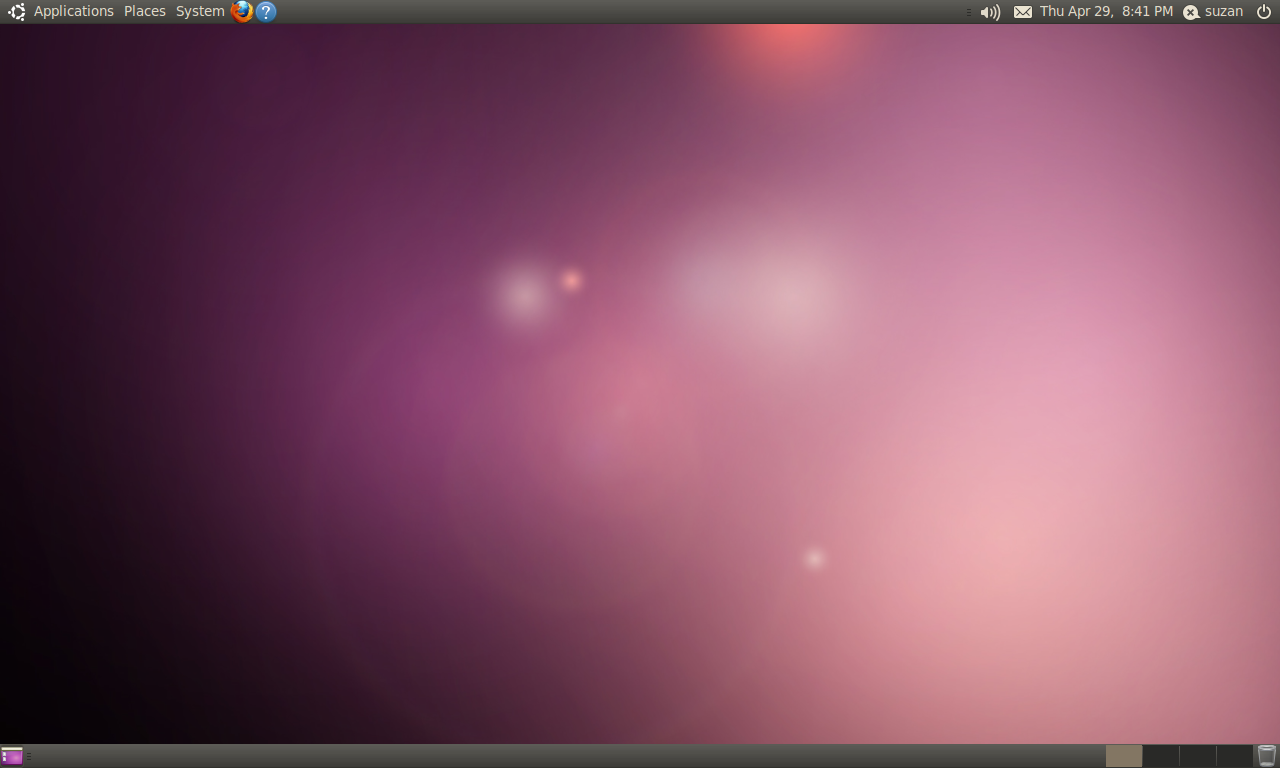
\includegraphics[width=400pt]{./images/ubuntu10-04.png}
	\caption{Ubuntu 10.04 Desktop}	
	\label{fig:ubuntu10.04}		
\end{figure}

\par \noindent In this section, only the changes are listed. How these new components work are covered in the upcoming chapters. \\

\begin{description}
	\item [Unity Launcher and Dash] Gone are the old application, places and systems menu. This is now replaced by the Unity dash and the launcher. Chapter \ref{chap:unity} will explain how to use them. But for now, it is important to understand the difference in launching and running applications between 10.04 and 12.04. This is one of the most important change which requires some time to get adjusted to.
	
	\item [Global Menu] In a bid to save vertical space, global menus are now part of the default 12.04 install. By default the application title is shown but when you hover over the top panel the global menu of the focussed application is shown. These is done to present a clean top panel appearance. 
		
	\item [HUD] Heads Up Display (HUD) is a new way accessing the menu items that you are looking for. It is currently present as a compliment to the Global menu. In the future, it will also provide support for voice commands. For a better understanding of HUD, please refer to chapter \ref{chap:unity}.

	\item [Gnome 3] Gnome 3 is now the new development focus of Gnome. This essentially means that every Gnome distribution will eventually upgrade to this new toolkit. With this toolkit, some features that were part of Gnome 2 are no longer supported. One such example is applets. Applets can no longer be added to the top panel. In Ubuntu 12.04, these are replaced by indicators. Many applets have already been converted into indicators which can be installed easily.	
\end{description}

\begin{figure}[h!]	
	\centering
	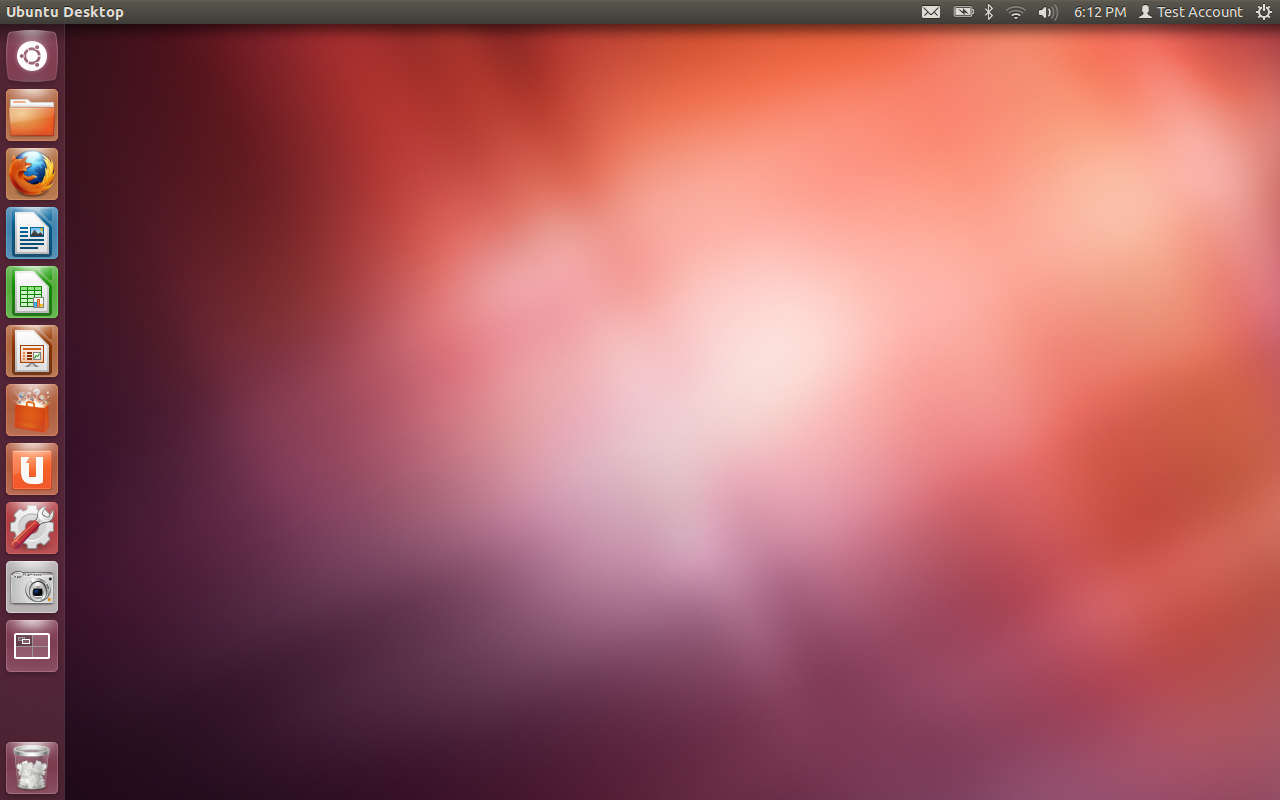
\includegraphics[width=400pt]{./images/ubuntu12-04.png}
	\caption{Ubuntu 12.04 Desktop}	
	\label{fig:ubuntu12.04}		
\end{figure}